\documentclass{elegantpaper}

\title{分布式空间top-k频繁关键字查询}

\author{
    冯运 1160300524 %
    \\[0.5ex] %
    陈进龙 1160300525 %
}

\begin{document}

\maketitle

\begin{abstract}
\end{abstract}

\section{问题描述}

随着社交软件的大量出现,许多社交平台允许用户在发布消息的时候会标记他们的地理位置,例如微博,微信朋友圈等.这样的背景条件下,就产生了新的数据分析问题.例如,当用户想去知道附近的热门地点时,需要对已经产生的地点信息进行计算,即用户给定一片空间区域,然后查询返回k个最热门的关键词,而随着数据产生的越来越多,数据量的存储已经远远超过了一个单机的能力,所以分布式的空间top-k关键字查询就成为了新的数据分析需求.

\subsection{形式化描述}
我们使用$L=\{o_1,o_2,o_3,...,o_n\} $ 来表示一个包含N个o对象的数据集,每一个对象$o_i$是<Place,Words>形式的对象.Place是一个n维的的空间坐标点,用$Place=\{w_1,w_2,...\}$来表示,而Words是对象o保存的关键字,用$Words=\{w_1,w_2,w_3... \}$.\newline
使用$V=\{U_{o\in L}O.Words\}$来表示L内的所有关键词的集合,使用$f_o(w)$来表示关键词$w$出现在对象o中的次数.\newline
对于一个给定的查询区域R,则可以用$f_R(w)=\{\sum{f_{oi(w)|o_i.Place\in R}} \}$来表示关键词w在区域R中出现的频率(次数).\newline
对于这个top-k频繁关键词查询系统来说,输入一个查询条件:$<R_Q,k>$,$R_Q$指明了选择的查询区域,k指明了最终输出的k个关键字,而这k个关键字是出现在$R_Q$区域内的k个最高频的关键字.\newline

\subsection{举例}

例如figure1表示的是一个二维的平面,其中包含了8个对象,则可以用$L=\{o_1,o_2,o_3,o_4,o_5,o_6,o_7,o_8\}$,每一个对象对应的关键词组在table1中展示
假设用户的查询是$Query=<R_4,3>$,即查询的区域是R4,用户要求的k=3的情况下,需要返回在区域R4中的top-3频繁的关键字,而从figure1中可以看出,在R4中包含的对象有$\{o_4,o_6,o_7,o_8\}$,根据table1可以算出最终的top-3为$\{w_2,w_3,w_9\}$.

\begin{figure}[!ht]
	\centering
	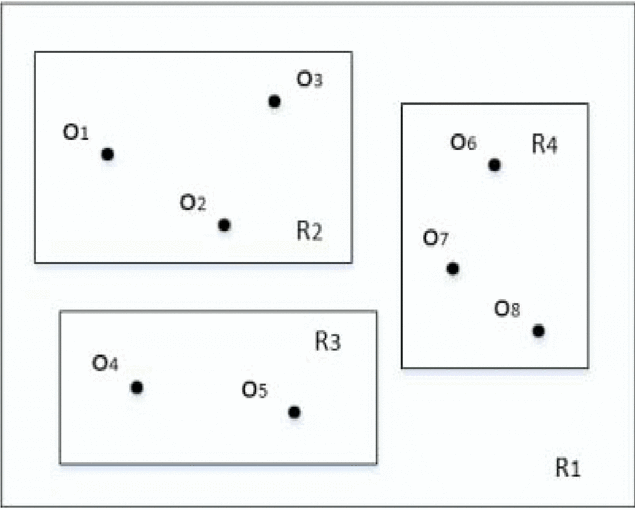
\includegraphics[width=0.6\textwidth]{figure1.png}
	\caption{空间示意图\label{fig:figure1}}
\end{figure}

\begin{table}[!htbp]
    \small
    \centering
    \caption{对象的}
      \begin{tabular}{cccc}
      对象&关键词&对象&关键词\\
      \hline
      $o_1$   & $\{w_2,w_3,w_5\}$ & $o_5$&$\{w_1,w_1,w_3,w_5\}$\\
      $o_2$   & $\{w_1,w_4,w_5\}$ & $o_6$&$\{w_4,w_7,w_9\}$\\
      $o_3$   & $\{w_2,w_4,w_4\}$ & $o_7$&$\{w_2,w_2,w_3,w_5\}$\\
      $o_4$   & $\{w_3,w_8,w_9,w_9\}$ & $o_8$&$\{w_3,w_3,w_6\}$\\
      \end{tabular}
\end{table}
  







\section{系统设计}

本节首先介绍一种分布式的索引结构,并基于此结构实现一种简单的查询算法。然后介绍基于此设计的一些改进以及相应的新的查询算法。

\subsection{分布式R树}

对于空间数据索引,首选的结构就是R树。但是传统的R树是基于单机的,没有考虑分布式计算的需求,故我们对R树做了一些改进,使其支持了分布式环境。
分布式R树的基本思想是将R树的节点与物理计算节点对应,即R树的一个节点存放在一个物理计算节点上。父节点所在的物理计算节点记录其所有子节点所包含的在的物理计算节点。

\subsubsection{内结点保存内容}

\begin{itemize}

    \item 本节点的MBR

    \item 子节点MBR集

    \item 每个子节点MBR对应的物理节点
    
\end{itemize}

\subsubsection{叶节点保存内容}

\begin{itemize}

    \item 本节点的MBR
    
    \item 在本区域出现的关键字列表,其中的项为形似\verb|<t, t.entries, t.freq>|的三元组,其中\verb|t|表示关键字,\verb|t.entries|为形似\verb|<loc, freq>|的二元组集合,表示\verb|t|出现的位置及在该位置出现的次数,\verb|t.freq|表示\verb|t|出现的总次数。

\end{itemize}

\subsection{索引创建}

在向索引集群导入数据的过程中,自动根据数据创建索引,具体过程如下:

\begin{itemize}
    
    \item[1.] 初始只有一个根节点服务器;
    
    \item[2.] 当数据量小于阈值$\delta$时,直接在根节点服务器上保存,即根服务器就作为唯一的叶节点;
    
    \item[3.] 当数据量大于等于阈值$\delta$时,向集群管理器申请新的多个新的计算节点,将数据按空间区域进行划分,并将划分后的数据分配到新申请的节点中,在本节点只保存划分信息;
    
    \item[4.] 

\end{itemize}

\subsection{执行查询}



\section{工作流程}

\end{document}